% Chapter 2

\chapter{Foundamentals of Machine Learning} % Main chapter title

\label{Chapter2} % For referencing the chapter elsewhere, use \ref{Chapter1} 

In this section, we introduce the basic of Machine learning.
In particular, we introduce the concepts of supervised learning, unsupervised learning, self-supervised learning and reinforcement leaning. 
We explain the difference between them and present some algorithms used for the thesis.
The reinforcement learning section is intended as introduction, while it will be deeply exposed in the next chapters.
For further details, refer to the body of Deep Learning\cite{goodfellow2016deep} 

\section{Introduction}

In its famous book, Tom Mitchell \cite{Mitchell97} provided widely quoted definitions of machine learning.
It says: "A computer program is said to learn from experience E with respect to some class of tasks T and performance measure P, if its performance at tasks in T, as measured by P, improves with experience E. For example, a computer program that learns to play checkers might improve its \textbf{performance} as measured by its ability to win at the class of \textbf{tasks} involving playing checkers games, through \textbf{experience} obtained by playing games against
itself."

Usually, machine learning algorithms are used for tasks that are too difficult to solve with fixed programs written by humans.
There are many classes of tasks that can be approached with machine learning, for example classification, regression, clustering, dimensionality reduction, data generation, machine translation, anomaly detection, denoising, density estimation.


For every task, there is a specific metric. The metric is a quantitative measure of the learner's abilities to solve the task, even for data that it has not seen before.   
Informally speaking, there are two main metrics.
The first one is the \textit{loss} that measures the model's error. For example for the classification task we could use a \textit{0-1 loss} that increment the total error rate by 0 when the input is correct classified and by 1 if it is none. 
The third is the \textit{reward} that is a feedback value that an agent receive every time it takes an action. It is positive when the action is correct and negative otherwise. So the performances of the agent depend on how much reward it is able to collect.

Machine learning algorithms can be classified by what kind of experience they are allowed to have in three main categories:
\begin{itemize}
\item \textbf{Supervised learning}: if all the model experience is concentrated in form of a given dataset in which every example is expressed by a vector of features. 
\item \textbf{Unsupervised learning}: where the examples in the dataset are not labelled.
\item \textbf{Reinforcement learning}: when the agent collect autonomously the experience in the dataset by interacting with the environment.
\end{itemize}

\section{Supervised Learning}
The problem that are faced with supervised learning are:
\begin{itemize}
\item \textbf{Classification}:  The classification problem consists of approximating a function $f:\mathbb{R}^n \rightarrow \left \{  1,...,k \right \}$ where k is the number of classes in which the dataset is divided.
This function $ y = f(x)$ will map every vector of features in which the input is represented to the corrected categories identified by category $y$.
\item \textbf{Regression}: In the regression task the program is asked to predict a continuous value relate to the input. So, in order to solve this task, the program should learn a function $f: \mathbb{R}^{n} \rightarrow \mathbb{R}$. 
\end{itemize}

It is time now to introduce a metric to evaluate algorithm performance. The task defines this metric.
For example, the loss function that we use for the classification task is the \textbf{cross entropy loss}. This metrics measures how the predicted distribution is close to the one that we are trying to approximate.
For the regression problem instead,  we could use the \textit{mean squared error} that increment the loss value proportionally to the distance between the correct answer and the model given value.

Once the model is trained, we want to know how it works with never seen before data to determine if the model has been capable of generalizing over the dataset. 
This ability is called \textbf{generalization}.

To do that, we divide the dataset into three parts:
\begin{itemize}
\item Train set: used for the training;
\item Validation set: used to evaluate the model and tune the parameters before a new training iteration;
\item Test set: used to calculate the final performance measure of the model;
\end{itemize}

It is essential to specify that the model does not see examples from the training's development and test set.

\subsection{Recurrent Neural Networks}
In this section, we briefly introduce the Recurrent Neural Network; for an extended explanation, see \cite{lipton2015critical}. This part is also based on the Understanding LSTM Networks blog post \cite{Colah}.\\

These models are called "neural networks" because they are inspired by neuroscience. As the biological version, the artificial neuron is modeled as a central nucleus connected with different inputs.
An artificial neuron's mathematical model is a weighted sum of the neuron connection $w_i$ and the respective input $x_i$.
$$a =w_{1} x_{1}+w_{2} x_{1}+w_{3} x_{3}+w_{i} x_{i}+\ldots+b=\sum_{i=0}^{i=N}\left(w_{i} x_{i}\right)+b$$We can rewrite more compactly the above formula using the matrix formulation: $ a = Wx + b$ . In order to produce the neuron output, the calculated weighted sum is passed through  a non-linear \textbf{activation function} $\Phi$. In that way the model acquire the ability to deal with more complex data respect to the one affordable by linear models.
$$ 
o=\Phi(a)=\Phi(\mathbf{W} \mathbf{x}+b)
$$
The early artificial neural model adopted the Sigmoid function as an activation function, but today the common choice is the Rectified Linear unit (\textbf{ReLu}).
Connecting various neurons allow the model to increase the representation power. In the neural networks, each neuron receives inputs from the others and uses it to calculate its activation value and propagate it. This network is divided into layers, each one that contains many neurons.
This architecture is called \textbf{Multilayer Perceptrons} (MLPs) or Feedforward network. 

In the MLP, the first layer is called \textbf{input layer} and receive the input.
The last one is called \textbf{output layer} and produces the output. 
All the intermediate layers are called \textbf{hidden layers}.
Feedforward neural network is a universal function approximation.
It defines a mapping $y = f(x;\theta)$ and learns approximate whatever function by merely learning the best set of parameter $\theta$.
These models can learn a hierarchical representation of the data, so they do not need hand-engineered features.
The training algorithm must use those hidden layers to produce the desired output, but the dataset does not contain explicit information on how to do that.\\

\begin{minipage}{\linewidth}
            \centering
            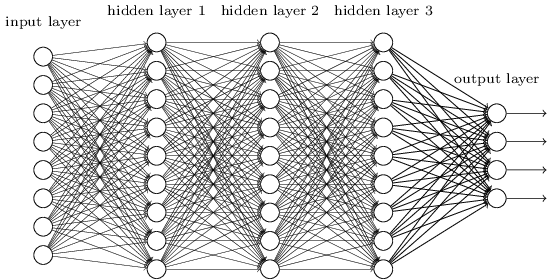
\includegraphics[width=.8\textwidth]{pictures/neural_network}
            \captionof{figure}{Fully-Connected Feed-Forward Network. Image from \cite{nielsenneural}.}
\end{minipage}


Neural network weights are trained with an algorithm called \textbf{Backpropagation}. The backpropagation algorithm is divided into two phases: a forward-pass and a backward-pass.
In the forward pass, the input is propagated throughout every layer and activation until the network's final output is computed. Then the error is calculated, calculating the difference between the network prediction and the training label. In the backward-pass, this error is backpropagated through all the layers to update each neuron's weights.  In the last layer, the update is obtained, calculating the error gradient to understand the change rate of the layer weights. For the hidden layers, instead, the chain rule is applied to propagate the gradient by decomposing the derivative of the produced error recursively with respect to the parameters of the previous layers. 
\\

The standard MLP model has some limitations. After each processed example, the full state of the network is lost. As long as the input data maintains temporal independence between them, there are no problems for learning.
Sometimes instead, the data is correlated, like with video frames or words in a sentence.
In that case, we need a model that can face these correlations even without knowing the input sequence length.
We can extend the "feedforward network," in which the path of the information strictly goes from input to the output by adding a feedback connection in which the information can go back to the model.
This extension allows us to introduce the notion of time to the model.
This new model is called a recurrent neural network (\textbf{RNN}).
In a RNN any state depend from both the current input and the network state in the previous time step.
Lastly, even if the expressive power grows exponentially, both the inference and training grow quadratically, and they are also differentiable end to end, so they are trainable with the backpropagation algorithm.
It is time now to introduce some details of the RNN.
We define a sequence of data as a arrays of data points $x^{(t)}$ extracted from a discrete sequence of \textit{time steps}, each one indexed by t and is expressed with real-valued vectors.
Both the input and the target are represented by a sequence ($x^{(1)},x^{(2)}, ..., x^{(T)}$).

\begin{figure}[h]
\centering
            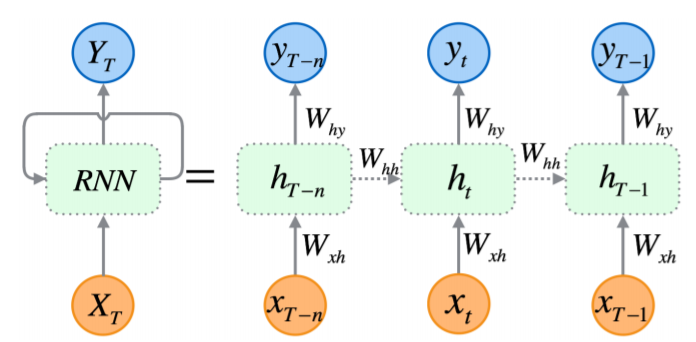
\includegraphics[width=.5\textwidth]{pictures/rnn_schema}
            \captionof{figure}{Standard RNN architecture and an unfolded structure with T time steps. Image from \cite{cui2018deep}.}
            \end{figure}

For each time step $t$ the current node receive information from both the data point $x^{t}$ in input and the previous state $h^{(t-1)}$ from the hidden node.
For each time step $t$, the current node receives information from both the input $x^{t}$ and the previous state $h^{(t-1)}$ and uses this information to update the current state $h^{(t)}$.
$$h^{(t)}=\sigma\left(W^{\mathrm{xh}} {x}^{(t)}+W^{\mathrm{hh}} {h}^{(t-1)}+{b}_{h}\right)$$
This current hidden state $h^{(t)}$ can be used to calculate the current output $y^{(t)}$.
$$\hat{y}^{(t)}=\operatorname{softmax}\left(W^{\mathrm{hy}} h^{(t)}+b_{y}\right)$$
The $W_{hx}$ is the matrix representing the weights from the input and the hidden layer.
The $W_{hh}$ is the matrix representing the recurrent weight between the same hidden layer through different time steps.
During the training, the error signal can be backpropagated through the entire unfolded network across all the time steps.
The backpropagation algorithm, used in a context where time is involved, is called \textit{backpropagation through time} (BPTT).
When we try to backpropagate the error across many time steps we can easily came across a problem of \textit{gradient exploding} or \textit{gradient vanishing}. One possible solution is to limits the maximum number of time steps in which the error can be backpropagated.
This solution is called Truncated backpropagation through time (TBTT).
Another solution is to design a particular architecture to limit the vanishing gradient problem without sacrifice the ability to learn long-range dependencies. 
This second approach led to a new neural network architecture called \textit{Long Short Term Memory} (\textbf{LSTM}) 


        \subsubsection{Long Short Term Memory}

In 1997 Hochreiter and Schmidhuber presented a new RNN architecture called Long Short-Term Memory (LSTM).
In this network, they introduce the memory cell, a new computational unit that replaces the traditional nodes in the network's hidden layers, to handle the vanishing gradient problem of the RNN.
In the traditional RNN, the long memory is maintained through the weights that capture the general knowledge about the data.
The short memory, instead, is represented by the activation function between each successive node.
In the LSTM, the memory cell works like intermediate storage and replaces short and long-term memory.
A memory cell is a composite unit that contains several gates that add or remove information to the cell state.
A gate is a sigmoidal unit that multiplies its output, between 0 and 1, with the value of another node to decide how much information can pass through.
We can describe the works of the LSTM through a sequence of 3 steps: 
\begin{enumerate}
\item \textbf{The Filter}: in the first step, the LSTM decides which information to accept as input and which to forget. To do that it uses the \textit{forget gate} that take in input the current input $x^{(t)}$ and the previous hidden layer $h^{(t-1)}$  and return a vector that will be used later to update the cell state. \\
\begin{minipage}{\linewidth}
            \centering
            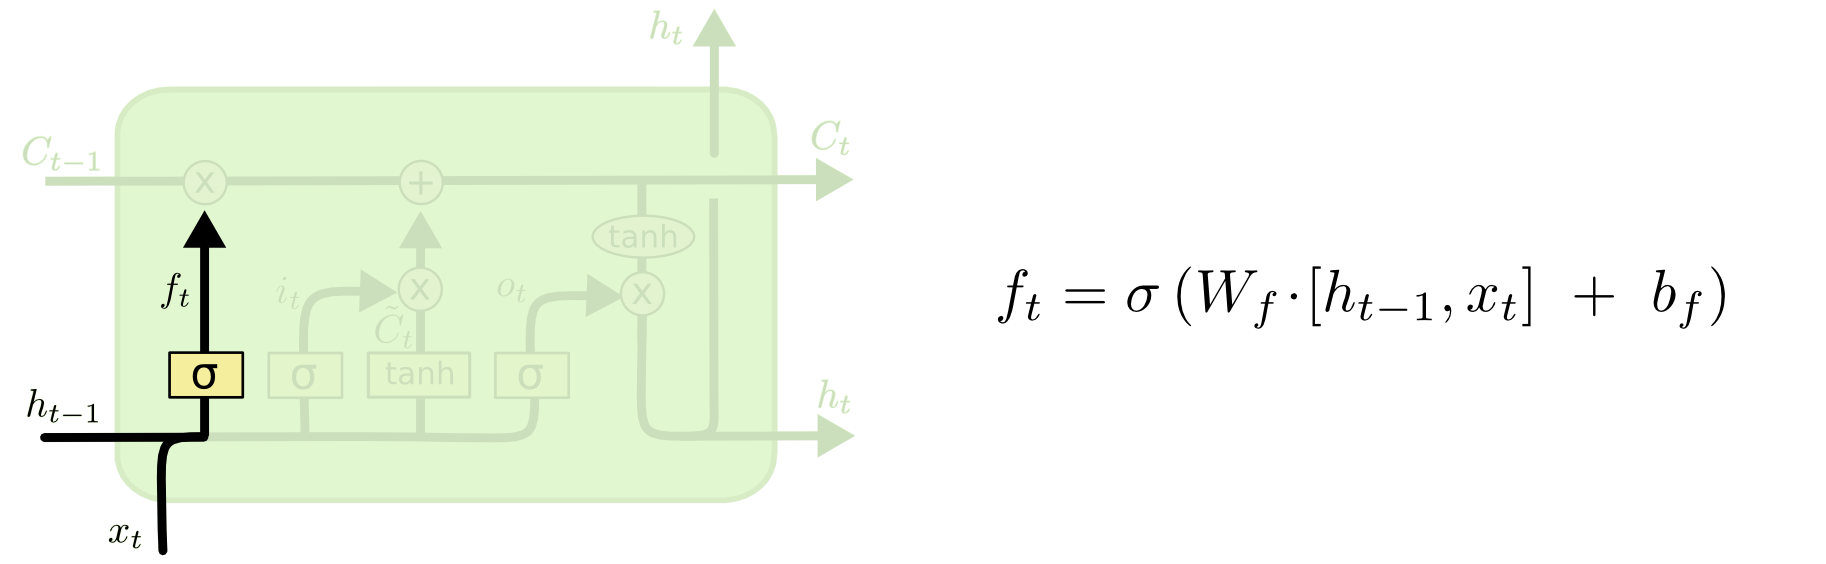
\includegraphics[width=10cm]{pictures/lstm_step1png}
            \captionof{figure}{The output of the sigmoid is a vector of values from zero (completely forget) to one (completely keep). Image from \cite{Colah}.}
        \end{minipage}
		

\item \textbf{The Update}: in the second step, the LSTM decides how much information store in the cell state. This step is divided into two parts: in the first one, it uses the \textit{input gate} to decide what value to update, and a tanh layer is used to create a vector of values called \textit{candidate values} that could be added to the state. In the second one, the LSTM updates its internal state, called \textit{Cell State}. 
			\begin{minipage}{\linewidth}
            \centering
            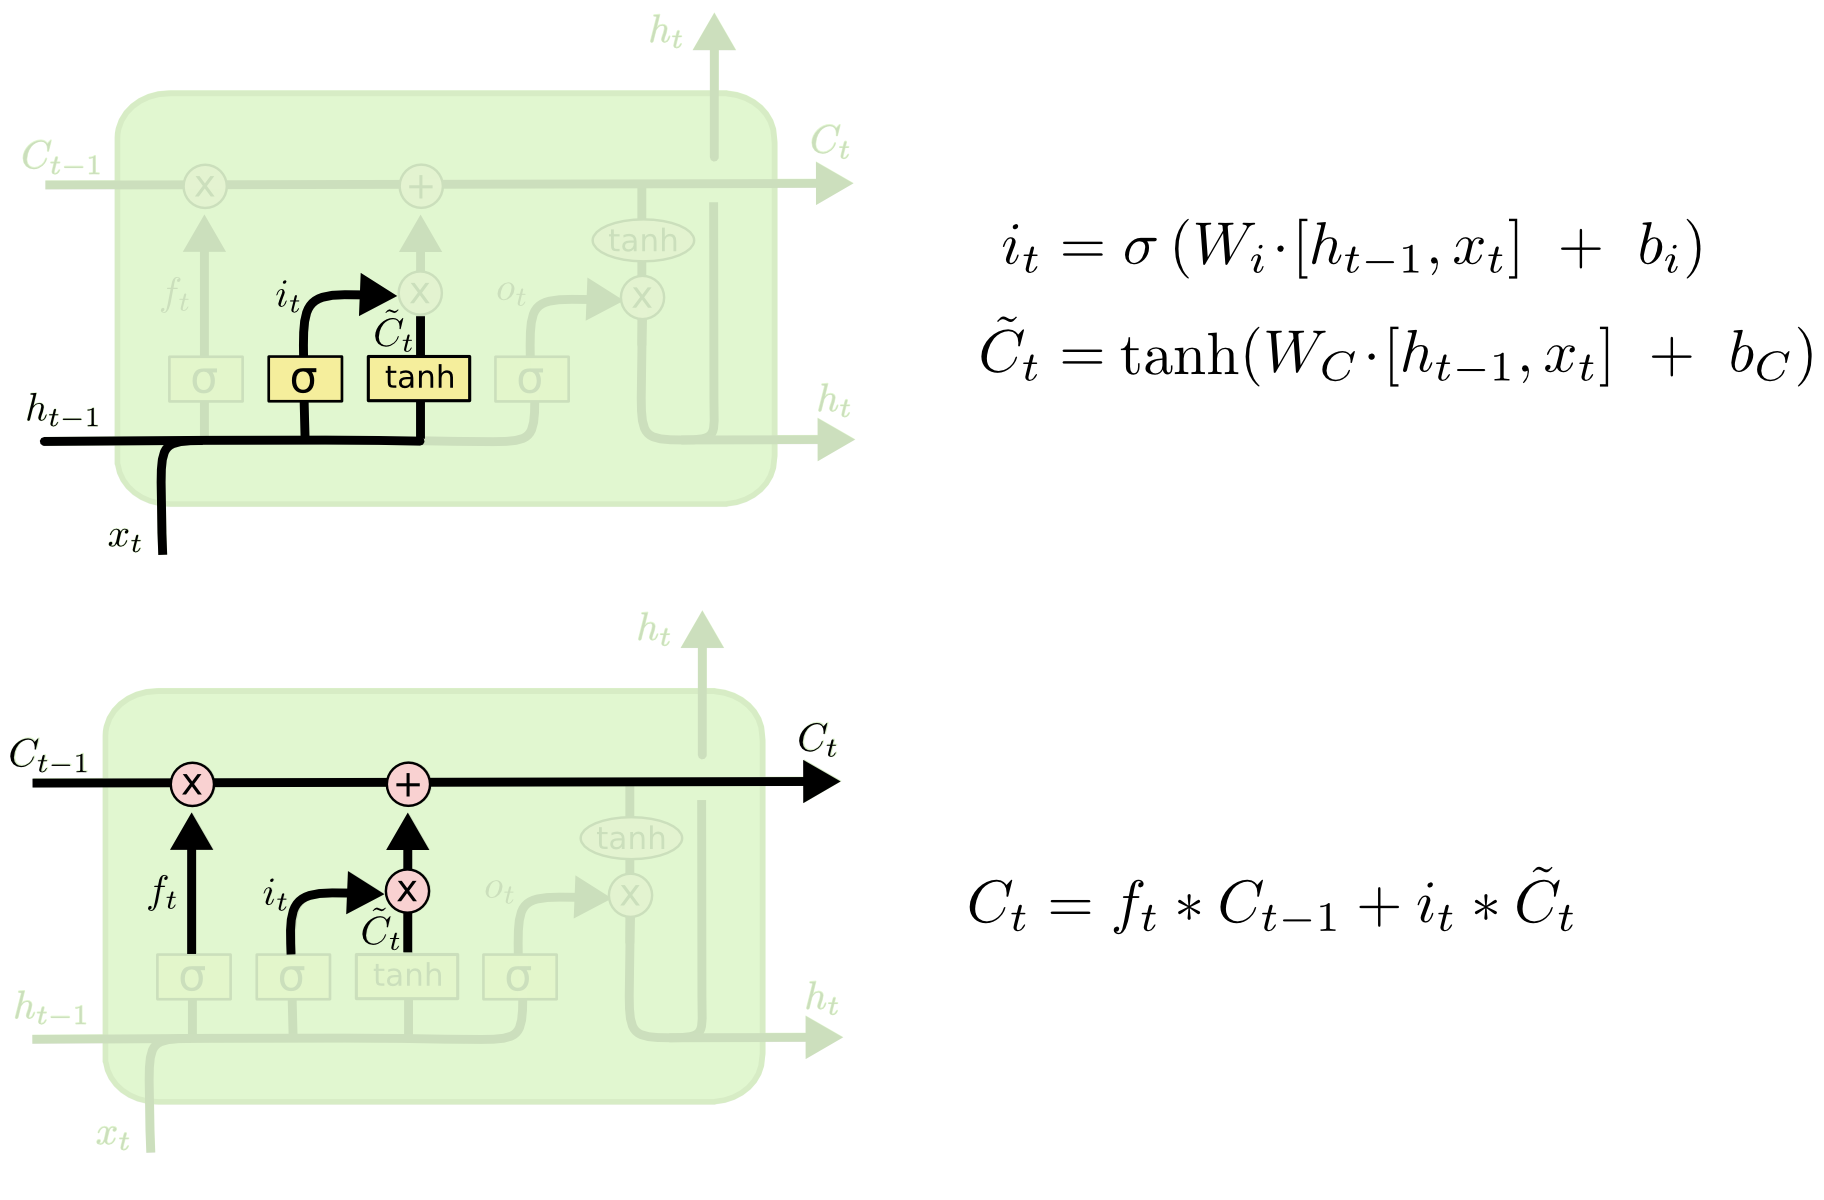
\includegraphics[width=10cm]{pictures/lstm_step2-3}
            \captionof{figure}{The Sigmod layer is used to decide what value to update, the Tanh layer to generate the vector of "candidate values" that could be added to the state. Next decides wich new information ignores, then in the tanh layer, it processes the new information respect the previously hidden layer and with the update gate decides which one to exclude for the update and which ti keep. Now it combines all this information to calculate the new Cell State. Image from \cite{Colah}.}
        \end{minipage}

\item \textbf{Compute Output}: in the final step, the LSTM combine previously hidden value, current input, and current cell state to calculate the new hidden value (that can be viewed as the current network's output). In this step, it is used the \textit{output layer} to decide what part of the state can be outputted.\\
\begin{minipage}{\linewidth}
            \centering
            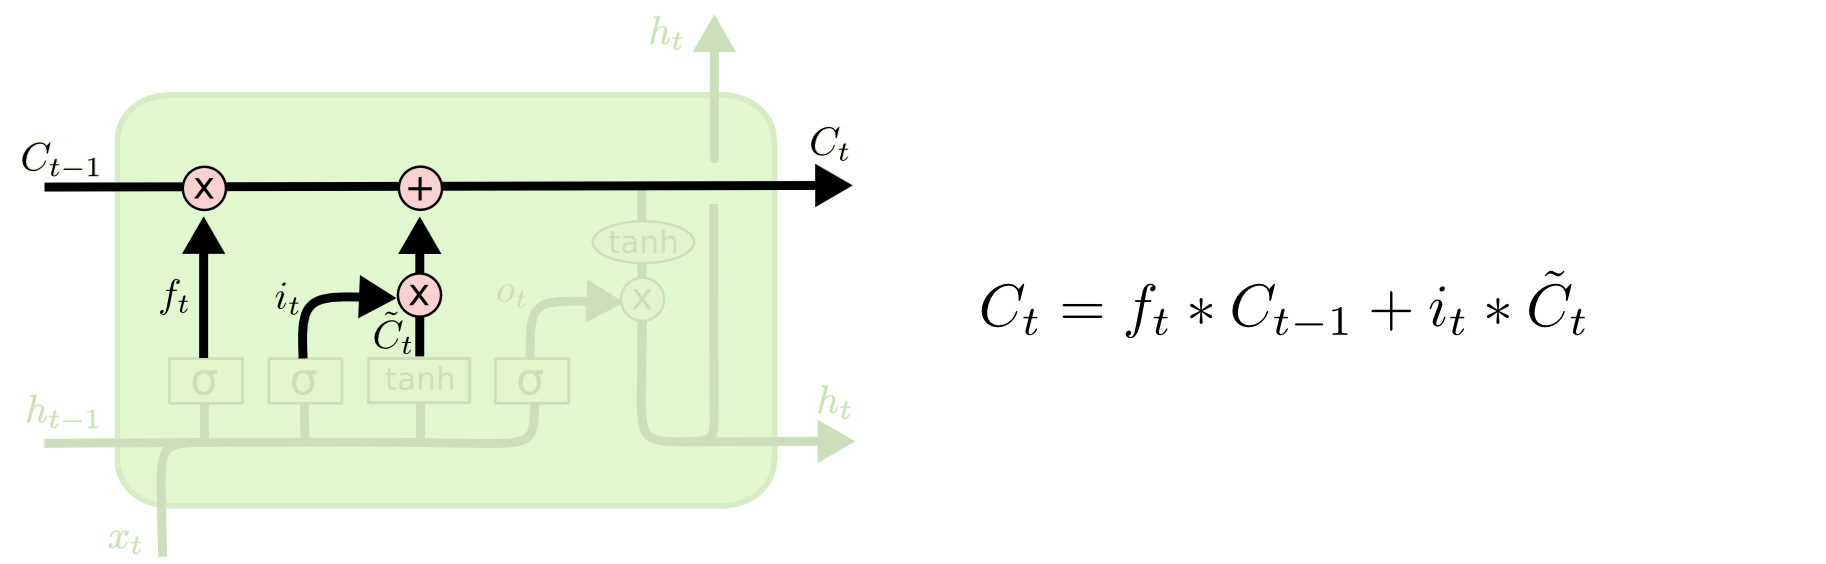
\includegraphics[width=10cm]{pictures/lstm_step3}
            \captionof{figure}{Use the internal state and the output gate to produce the new hidden state. Image from \cite{Colah}.}
\end{minipage}

\end{enumerate}
The LSTM is still used since they have shown a better ability to handle long-range dependencies with respect to the simple RNNs.

\begin{minipage}{\linewidth}
            \centering
            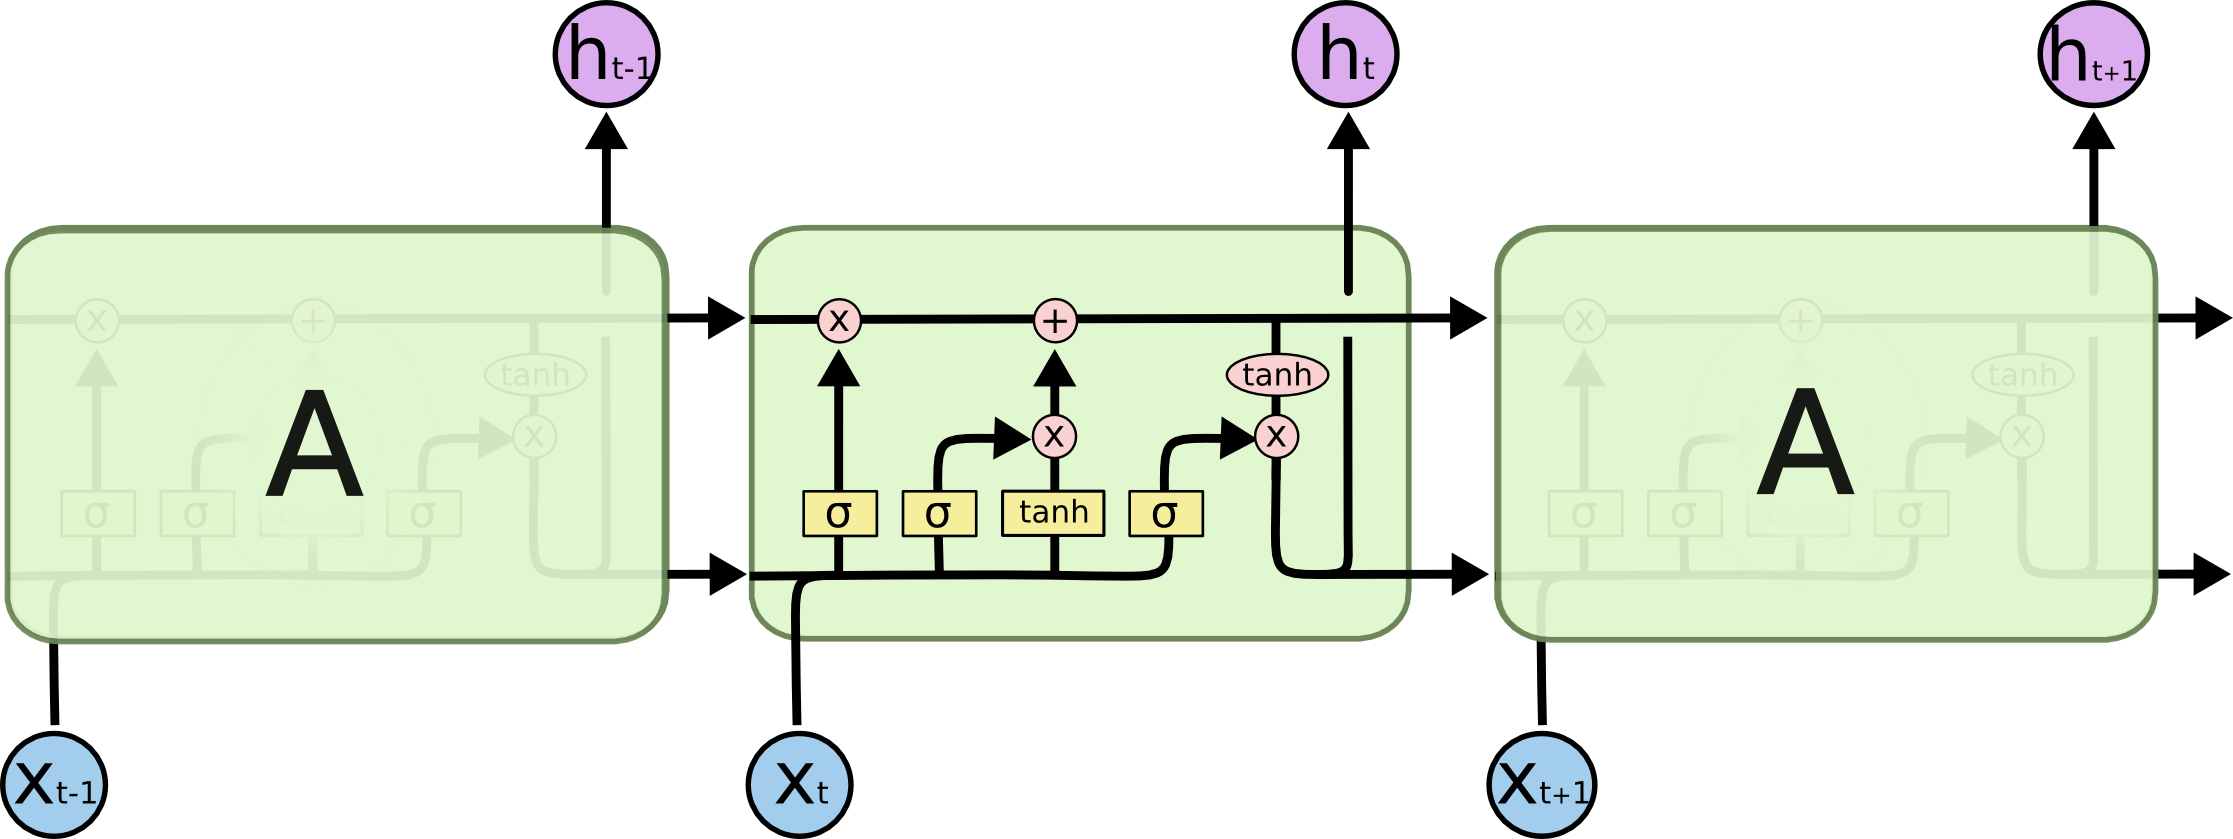
\includegraphics[width=1.0\textwidth]{pictures/lstm_final}
            \captionof{figure}{The LSTM architecture consist on a concatenation of LSTM cell units. Image from \cite{Colah}.}
\end{minipage}


\section{Unsupervised Learning}
The principal tasks of unsupervised learning are:
\begin{itemize}
    \item \textbf{Clustering}: is used to automatically dividing the dataset into clusters of a similar example.
    \item \textbf{Dimensionality Reduction}:  reducing the number of observed random variables in a reduced set of principal variables.
\item \textbf{Generative models}: learning a joint distribution over all the variables. In other words, a generative model simulates how the data is generated in the real world.
\end{itemize}

Recently a new subsets of Unsupervised learning methods has been introduce by Yann LeCun in and it is call \textbf{Self-supervised Learning}. 
According with Longlong Jing and Yingli Tian \cite{jing2020self} 

Self-supervised learning follow the same principle of provide to the learning algorithm a set of pair $X_i$ and $Y_i$ but with the difference that $Y_i$  are automatically generated without involving human annotations. That labels are called psuedo labels.
We introduce one example of this technique: the \textbf{Variational Autoencoder}.

\subsection{Variational  Autoencoder}
Variational  Autoencoder is an example of the class of \textbf{generative model} methods.
Here we provide a general explanation based on the introductory paper \cite{kingma2019introduction}.

In a generative model setting, we try to estimate, explicitly or implicitly, a probability distribution of the data.
Once the generative model has been tuned or trained, we can sample from the estimated distribution and we can generate new input data samples.
The VAE is an implicit generative model, because it produces its own internal representation of the data without producing an explicit formula for the data probability distribution.
For this reason, this model is also used as a method to build a more compact representation of the data, minimizing the information loss.
For the experiments in chapter \ref{Chapter6}, the VAE is used both as a dimensionality reduction algorithm and a generative model.

The VAE represents the marginal distribution over the samples with a function $p_\theta(x|z)$ parameterized with $ \theta $.
This probability is conditionally dependent on the latent variable z.
\begin{equation*}
p_\theta(x) = \int p_\theta(x,z)dz =\int p_\theta(x |z) p(z)dz .
\end{equation*}If we are in a discrete case (so if $z$ is a discrete variable), and $p_\theta(x|z)$ is assumed to be a Gaussian distribution, then $p_\theta(x)$  is a Gaussian mixture distribution.
Instead, if we are working with a continuous variable z, then $p_\theta(x)$ can be seen as an infinite Gaussian mixture distribution.
In this work $z$ is a continuous vector described by a simple Gaussian distribution and $p_\theta(x|z)$ is a conditional Gaussian. 

We need a function that takes all the data in training set as inputs and extract from them the parameters of the latent Gaussian.
Then we can sample the latent vector z from this latent Gaussian.  
We call this function \textbf{encoder} and we formally define it as:
\begin{equation*}
q_\phi(z|x) = \mathcal{N}(\mu_\phi(x),\sigma_\phi(x))
\end{equation*}
Then we need also another function that uses this latent vector z to retrieve x.
We call this function \textbf{decoder} and we formally define it as:
\begin{equation*}
p_\theta(x|z) = \mathcal{N}(\mu_\theta(z),\sigma_\theta(z))
\end{equation*}
In order to find the best parameters $\theta$ we would like to use the Maximum Likelihood principle that is:
\begin{equation}
\label{intractable}
\theta \leftarrow \arg \max_{\theta} \frac{1}{N} \sum_{i} \log \left ( \int p_\theta(x_i|z)p(z)dz \right ).
\end{equation}
Unfortunately, this formula is completely intractable, because of the integral in $ \log\, p(x_i) = \log \int_z p(x_i|z) \, p(x)$, so we need another way.

Before moving on we introduce two concepts that we will use later: entropy and the Kullback-Leibler divergence.

\textbf{Entropy}:  introduced in 1948 by Claude Shannon, the entropy measures the level of uncertainty of a stochastic variable outcome.
For example, an event that has the high probability of occurring, say 90\%, do not give us much information, so it has low entropy.
Instead if we A coin instead, in which all the events have the same probability, will have a high level of entropy.
The formula of the entropy is:
\begin{equation*}
\mathcal{H} = -E_{x\sim p(x)} \left [ \log\, p(x) \right] = - \int_{x} p(x) \log \,p(x) dx
\end{equation*}
\textbf{KL-Divergence}: is a measure of how well a distribution Q approximates another probability P, or in other words, how much information it's lost if the distribution Q is used instead of P.
\begin{equation*}
D_{KL} (P||Q) = E_{x \sim P} \left [ \log \frac{P(x)}{Q(x)} \right] 
\end{equation*}

\begin{itemize}
\item Notice that it is not a distance between two distribution because is not symmetric:\begin{equation*}
 D_{KL}(P || Q) \neq D_{KL}(Q|| P)
 \end{equation*}
\item Where P=Q the KL-divergence is 0:\begin{equation*}
 log  \frac{P}{Q} = log 1 = 0
 \end{equation*}
\item The KL- divergence is always a positive number.
\end{itemize}

Now we can go back to the VAE.
The encoder part is represented by a neural network with parameters $w$, trained to approximate the latent distribution $q_\phi$.
In other words, this neural network will find, from all the training examples x, the respective Gaussian parameters for the latent vector.
So, more formally:
\begin{equation*}
q(z) =  \hat{q}_w(z|x) \approx q_\phi(z|x) 
\end{equation*}
As we have seen before in equation \ref{intractable} it is not possible to use directly that formula.
We need to find another way to define the $\log \, p_\theta(x)$:
\begin{equation*}
    \log\,{p_\theta (x)} = \mathbb{E}_{q_\phi (z|x)} \left[ \log \, p_\theta (x) \right]
\end{equation*}
Now we apply the Bayes's theorem:
\begin{equation*}
p_\theta(x) = \frac{p_\theta(x|z)p_\theta(z)}{p_\theta(z|x)} = \frac{p_\theta(x,z)}{p_\theta(z|x)}
\end{equation*}
and substitute the $p_\theta$(x):


\begin{equation*}
      \log\,{p_\theta (x)} = \mathbb{E}_{q_\phi (z|x)} \left[ \log \left( \frac{p_\theta(x,z)}{p_\theta(z|x)} \right) \right]
\end{equation*}
now we multiply by a constant $q_\phi (z|x)$ (the distribution of the encoder):
\begin{equation*}
      \log\,{p_\theta (x)} = \mathbb{E}_{q_\phi (z|x)} \left[ \log \left( \frac{p_\theta(x,z)}{q_\phi(z|x)} \, \frac{q_\phi(z|x)}{p_\theta(z|x)} \right) \right].
\end{equation*}
next we decompose the expected value:
\begin{equation*}
\log\,{p_\theta (x)} = \mathbb{E}_{q_\phi (z|x)} \left[ \log \left( \frac{p_\theta(x,z)}{q_\phi(z|x)} \right) \right] + \mathbb{E}_{q_\phi (z|x)} \left[ \log \left( \frac{q_\phi(z|x)}{p_\theta(z|x)} \right) \right].
\end{equation*}
We can rewrite the second term as the KL-divergence between $q_\phi$ e $p_\theta$:
\begin{equation*}
\mathbb{E}_{q_\phi (z|x)} \left[ \log \left( \frac{q_\phi(z|x)}{p_\theta(z|x)} \right) \right] = D_{KL} \left ( q_\phi(z|x)||p_\theta(z|x) \right ).
\end{equation*}
Now we focus on the first term:
\begin{align*}
\mathbb{E}_{q_\phi (z|x)} & \left[ \log \left( \frac{p_\theta(x,z)}{q_\phi(z|x)} \right)\right]
\end{align*}
we rewrite the joint probability as a conditional probability:

\begin{align*}
\mathbb{E}_{q_\phi (z|x)} & \left[ \log \left( \frac{p_\theta(x|z)p_\theta(z)}{q_\phi(z|x)} \right)\right]
\end{align*}
we apply the property of logarithms:

\begin{align*}
\mathbb{E}_{q_\phi (z|x)} & \left[ \log\,p_\theta(x|z) \right] -  \mathbb{E}_{q_\phi (z|x)} \log \left ( \frac{q_\phi(z|x)}{p_\theta(z)}   \right)
\end{align*}
we rewrite the second element as a KL-divergence
\begin{align*}
\mathbb{E}_{q_\phi (z|x)} & \left[ log\,p_\theta(x|z) \right] - D_{KL}(q_\phi(z|x)||p_\theta(z))
\end{align*}
Now we can rewrite the entire formula as:
\begin{equation*}
\log_{p_\theta}(x) = \underbrace{\mathbb{E}_{q_\phi(z|x)}[\log \, p_\theta(x|z)]}_{\text=Reconstruction \, error} - \underbrace{D_{KL}(q_\phi(z|x)||p_\theta(z))}_{\text=First \, regularization \, term} + \underbrace{D_{KL}(q_\phi(z|x)||p_\theta(z|x))}_{\text=Second \, regularization \, term}
\end{equation*}
Let us now examine all the components of the formula one by one.

Let's start with the first regularization term. 
It represents the similarity between the encoder and the latent distribution. 
Since both are Gaussians it is possible to calculate the KL in a closed form.

\begin{equation*}
KL(p||q) = \frac{1}{2} \left[ log \frac{\Sigma_2}{\Sigma_1} -d + tr(\Sigma_{2}^{-1}\Sigma_1) + (\mu_2 - \mu_1)^T \Sigma_{2}^{-1} (\mu_2 - \mu_1)\right]
\end{equation*}
The second regularization term instead, represents the similarity between the encoder and the true posterior $p(z|x)$ but it is not possible to calculate it.

We know that the KL divergence is always positive, so we can ignore the second regularization term and obtain a computable lower bound of the $\log\,p_\theta(x)$  that is called Expected Lower BOund (ELBO). 

% RIPARTIRE DA QUI%%
Lastly, we need to find a way to calculate the Reconstruction error term.
This term is the decoder's contribution to the final result: the ability to rebuild x given the latent vector z.
We can approximate it through the sampling and SGD optimization, but we need to introduce a little trick before, called "\textbf{the reparametrization trick}."

We divide the training time into two-phase: forward propagation and backpropagation.

In the forward phase, the encoder produces the parameters for the latent distribution from the given input.
From this distribution, the latent vector is sampled and given to the decoder.
The decoder uses this vector to recreate the original input.
The difference between the decoder's output and the original input is the error of the VAE, and it must be backpropagated for all the computational graph.

In the backpropagation phase, the error passes through the decoder but fails to reach the encoder.
That is because the sampling of z is a non-continuous and a non-differentiable operation; it has no gradient.
So we need to make deterministic the choice of z but to keep stochasticity by applying the reparametrization trick.

\begin{figure}[h]
\centering
\label{reparameterization_trick}
     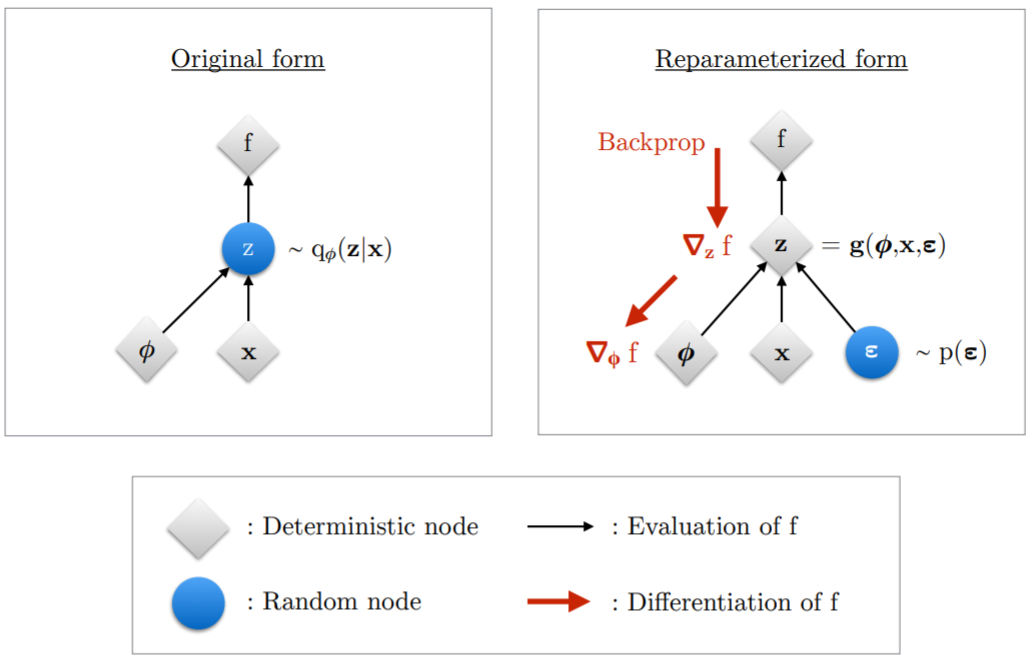
\includegraphics[width=1.0\textwidth]{pictures/reparameterization_trick}
      \caption{Illustration of the reparameterization trick.}
\end{figure}
This method consists of adding a new parameter called $\epsilon$  that is randomly sampled, but that is independent of encoder parameters $\phi$.
\begin{equation*}
\epsilon \sim \mathcal{N}(0,1)
\end{equation*}
Since we cannot directly backpropagate the gradients through the vector z because of its randomness, we re-parameterizing this variable z as deterministic and differentiable.

Now the latent vector is no more sampled but computed:
\begin{equation*}
z = \mu_\phi (x) + \epsilon\sigma_\phi(x)
\end{equation*}
The expectations can be rewritten in terms of $\epsilon$:
\begin{equation*}
\mathrm{E}_{q_\phi(z|x)}[f(z)] = \mathrm{E}_{p(\epsilon)}[f(z)]
\end{equation*}
where $z = g(\epsilon, \phi, x)$.
Finally it is possible to calculate $\nabla_\phi  g(\phi,x,\epsilon)$

\begin{figure}[h]
\centering
     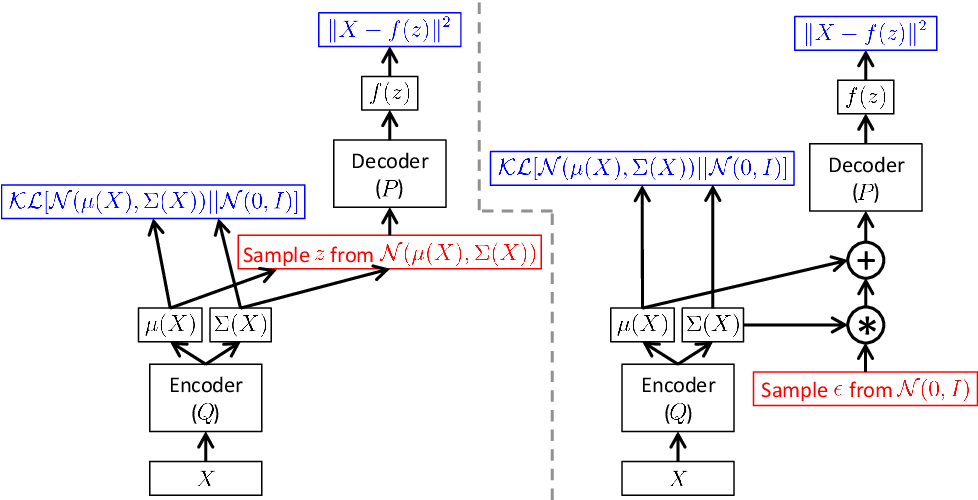
\includegraphics[width=1.0\textwidth]{pictures/vae_struct}
      \caption{A training-time variational autoencoder implemented as a feedforward neural network, where P(X|z) is Gaussian. Left is without the “reparameterization trick”, and right is with it. Image from \cite{doersch2016tutorial}.}
\end{figure}


\section{Reinforcement Learning}
In the reinforcement learning scenario the learner is an agent in an environment. The agent that does not know the environment dynamics, what its purpose is, and obviously how to achieve it.
However, it can choose an action and perform it, and then it will receive a feedback signal that it will use to understand if it was a good or bad action. 

There are infinite possible environments, and for each of them, there are infinite possible objectives. 
Therefore it is necessary to build a method capable of learning in a given environment without any supervision.
The agent's objective function is independent of the environment and it is universal, so it is always the same.
Each agent maximizes the feedback signal and indirectly, in doing so, solves the environment.
The feedback signal is built in such a way that, maximizing it, will lead to resolving the environment. 

Reinforcement learning also differs from unsupervised learning because while the first one is about to maximize a reward signal, the second one is about finding the hidden structure in the collection of unlabeled data.
In the following chapter we explain in more detail the reinforcement learning theory with an explanation of the mathematical preliminaries associated with it.




